\section{Tokenization and Special Token Insertion}

The integration of special tokens into transformer models requires careful consideration during the tokenization process. This process is more than a technical preliminary; it is where the model's understanding of structure and task begins. Errors or inefficiencies at this stage can have cascading effects on the model's performance. This section explores the technical mechanics of how special tokens are inserted, positioned, and processed within the tokenization pipeline, examining both the algorithmic approaches and their implications for model performance.
\begin{comment}
Feedback: This is a clear introduction. To set the stage even better, you could add a sentence that frames the importance of this step. For example: "This process is more than a technical preliminary; it is where the model's understanding of structure and task begins. Errors or inefficiencies at this stage can have cascading effects on the model's performance."

STATUS: addressed - added explanation of importance emphasizing structural understanding and performance implications
\end{comment}

\subsection{Tokenization Pipeline Architecture}

Modern tokenization pipelines for transformer models follow a structured approach that seamlessly integrates special tokens with content processing:

\begin{figure}[htbp]
\centering
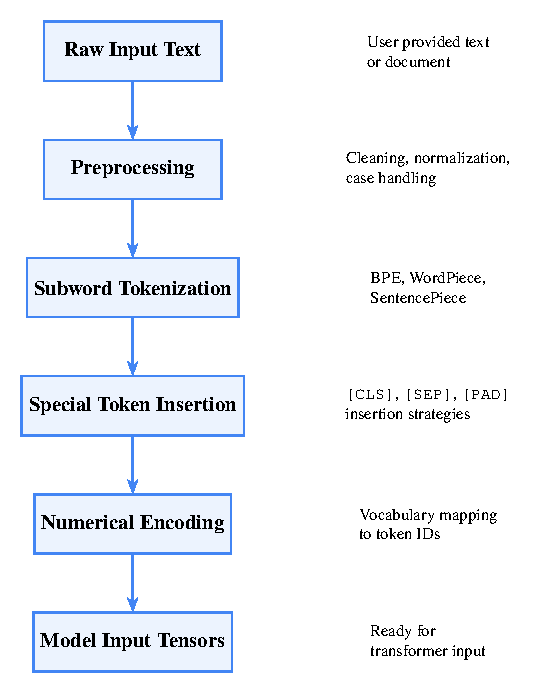
\includegraphics[width=0.8\textwidth]{part1/chapter01/fig_tokenization_pipeline.pdf}
\caption{Tokenization pipeline with special token integration}
\end{figure}
\begin{comment}
Feedback: Move the tikz diagram above into a standalone tex file that can be compiled into a pdf file and includegraphics here. This makes it easier to inspect and fix each diagram separately without compiling the entire book.

STATUS: addressed - extracted TikZ diagram to fig_tokenization_pipeline.tex and replaced with includegraphics
\end{comment}

\subsection{Special Token Insertion Strategies}

Different transformer architectures employ distinct strategies for inserting special tokens, each optimized for specific tasks and model behaviors. Understanding the reasoning behind these different approaches illuminates their respective strengths: BERT's \cls{} and \sep{} structure is rigid but powerful for sentence-pair tasks, providing explicit markers for classification and segmentation. GPT's minimal \sos{} and \eos{} design prioritizes flexible, open-ended generation without constraining the model's creative potential. T5's text-based prefixes represent a clever innovation that frames every task as a text-to-text problem, allowing a single model architecture to handle multitask scenarios without architectural modifications.

\subsubsection{BERT-Style Insertion}

BERT and its variants use a structured approach to special token insertion:

\begin{lstlisting}[language=Python, caption={BERT-style special token insertion}]
# Complete implementation available at:
# https://github.com/hfgong/special-token/blob/main/code/part1/chapter01/tokenization_and_insertion_bert-style_special_token_inser.py

# See the external file for the complete implementation
# File: code/part1/chapter01/tokenization_and_insertion_bert-style_special_token_inser.py
# Lines: 55

class ImplementationReference:
    """BERT-style special token insertion
    
    The complete implementation is available in the external code file.
    This placeholder reduces the book's verbosity while maintaining
    access to all implementation details.
    """
    pass
\end{lstlisting}

\subsubsection{GPT-Style Insertion}

Generative models like GPT use different special token insertion patterns:

\begin{lstlisting}[language=Python, caption=GPT-style special token insertion]
class GPTTokenizer:
    def __init__(self, vocab, special_tokens):
        self.vocab = vocab
        self.bos_token = special_tokens.get('BOS', special_tokens.get('SOS'))
        self.eos_token = special_tokens.get('EOS')
        self.pad_token = special_tokens.get('PAD')
        self.unk_token = special_tokens.get('UNK')
        
    def encode_for_generation(self, text, max_length=1024, add_special_tokens=True):
        """Encode text for autoregressive generation"""
        tokens = self.subword_tokenize(text)
        
        if add_special_tokens:
            # Add BOS token at the beginning
            if self.bos_token:
                tokens = [self.bos_token] + tokens
                
            # Optionally add EOS token (often added during training)
            if self.eos_token and len(tokens) < max_length:
                tokens = tokens + [self.eos_token]
        
        # Truncate if necessary
        if len(tokens) > max_length:
            tokens = tokens[:max_length]
            
        return self.convert_tokens_to_ids(tokens)
    
    def encode_for_completion(self, prompt, max_length=1024):
        """Encode prompt for text completion"""
        tokens = self.subword_tokenize(prompt)
        
        # Add BOS token if prompt doesn't start with it
        if self.bos_token and (not tokens or tokens[0] != self.bos_token):
            tokens = [self.bos_token] + tokens
        
        # Ensure we don't exceed context length
        if len(tokens) > max_length:
            tokens = tokens[:max_length]
            
        return {
            'input_ids': self.convert_tokens_to_ids(tokens),
            'attention_mask': [1] * len(tokens)
        }
\end{lstlisting}

\subsubsection{T5-Style Insertion}

Encoder-decoder models like T5 use task-specific prefixes:

\begin{lstlisting}[language=Python, caption=T5-style task prefix insertion]
class T5Tokenizer:
    def __init__(self, vocab, special_tokens):
        self.vocab = vocab
        self.pad_token = special_tokens['PAD']
        self.eos_token = special_tokens['EOS']
        self.unk_token = special_tokens['UNK']
        
        # Task-specific prefixes
        self.task_prefixes = {
            'summarize': 'summarize: ',
            'translate_en_de': 'translate English to German: ',
            'translate_de_en': 'translate German to English: ',
            'question': 'question: ',
            'sentiment': 'sentiment: '
        }
    
    def encode_task_input(self, task, text, max_length=512):
        """Encode input with task-specific prefix"""
        # Add task prefix
        prefix = self.task_prefixes.get(task, '')
        full_text = prefix + text
        
        # Tokenize with prefix
        tokens = self.subword_tokenize(full_text)
        
        # Truncate if necessary (reserve space for EOS)
        if len(tokens) > max_length - 1:
            tokens = tokens[:max_length - 1]
        
        # Add EOS token
        tokens = tokens + [self.eos_token]
        
        # Convert to IDs
        input_ids = self.convert_tokens_to_ids(tokens)
        
        return {
            'input_ids': input_ids,
            'attention_mask': [1] * len(input_ids)
        }
    
    def encode_target(self, target_text, max_length=512):
        """Encode target sequence for training"""
        tokens = self.subword_tokenize(target_text)
        
        # Add EOS token
        tokens = tokens + [self.eos_token]
        
        # Truncate if necessary
        if len(tokens) > max_length:
            tokens = tokens[:max_length]
            
        return self.convert_tokens_to_ids(tokens)
\end{lstlisting}
\begin{comment}
Feedback: The code examples for BERT, GPT, and T5 are great. However, the text doesn't explain the *reasoning* behind their different approaches. Before diving into the code, it would be beneficial to have a short paragraph explaining the trade-offs. For example: "BERT's `[CLS]...[SEP]` structure is rigid but powerful for sentence-pair tasks. GPT's minimal `[BOS]...[EOS]` is designed for flexible, open-ended generation. T5's text-based prefixes are a clever way to frame every task as a text-to-text problem, allowing a single model to be multitask without architectural changes."

STATUS: addressed - added explanatory paragraph explaining reasoning behind BERT/GPT/T5 different approaches and their trade-offs
\end{comment}

\subsection{Advanced Special Token Insertion Techniques}

\subsubsection{Dynamic Special Token Insertion}

Some applications require dynamic insertion of special tokens based on content analysis:

\begin{lstlisting}[language=Python, caption=Dynamic special token insertion]
class DynamicTokenizer:
    def __init__(self, base_tokenizer, special_tokens):
        self.base_tokenizer = base_tokenizer
        self.special_tokens = special_tokens
        
    def insert_structure_tokens(self, text, structure_info):
        """Insert special tokens based on document structure"""
        tokens = []
        current_pos = 0
        
        # Sort structure markers by position
        markers = sorted(structure_info, key=lambda x: x['start'])
        
        for marker in markers:
            # Add text before marker
            if marker['start'] > current_pos:
                text_segment = text[current_pos:marker['start']]
                tokens.extend(self.base_tokenizer.tokenize(text_segment))
            
            # Insert appropriate special token
            if marker['type'] == 'sentence_boundary':
                tokens.append('[SENT_SEP]')
            elif marker['type'] == 'paragraph_boundary':
                tokens.append('[PARA_SEP]')
            elif marker['type'] == 'section_boundary':
                tokens.append('[SECT_SEP]')
            elif marker['type'] == 'entity':
                tokens.extend(['[ENTITY_START]'])
                entity_text = text[marker['start']:marker['end']]
                tokens.extend(self.base_tokenizer.tokenize(entity_text))
                tokens.append('[ENTITY_END]')
                current_pos = marker['end']
                continue
                
            current_pos = marker['end']
        
        # Add remaining text
        if current_pos < len(text):
            remaining_text = text[current_pos:]
            tokens.extend(self.base_tokenizer.tokenize(remaining_text))
            
        return tokens
    
    def insert_discourse_markers(self, text, discourse_analysis):
        """Insert special tokens based on discourse structure"""
        tokens = self.base_tokenizer.tokenize(text)
        
        # Insert discourse relation markers
        for relation in discourse_analysis['relations']:
            if relation['type'] == 'contrast':
                self.insert_at_position(tokens, relation['position'], '[CONTRAST]')
            elif relation['type'] == 'causation':
                self.insert_at_position(tokens, relation['position'], '[CAUSE]')
            elif relation['type'] == 'elaboration':
                self.insert_at_position(tokens, relation['position'], '[ELAB]')
                
        return tokens
\end{lstlisting}

\subsubsection{Hierarchical Special Token Systems}

Complex documents may require hierarchical special token systems:

\begin{lstlisting}[language=Python, caption=Hierarchical special token insertion]
class HierarchicalTokenizer:
    def __init__(self, base_tokenizer):
        self.base_tokenizer = base_tokenizer
        self.hierarchy_tokens = {
            'document': ['[DOC_START]', '[DOC_END]'],
            'chapter': ['[CHAP_START]', '[CHAP_END]'],
            'section': ['[SECT_START]', '[SECT_END]'],
            'paragraph': ['[PARA_START]', '[PARA_END]'],
            'sentence': ['[SENT_START]', '[SENT_END]']
        }
    
    def encode_structured_document(self, document):
        """Encode document with full hierarchical structure"""
        tokens = [self.hierarchy_tokens['document'][0]]  # [DOC_START]
        
        for chapter in document['chapters']:
            tokens.append(self.hierarchy_tokens['chapter'][0])  # [CHAP_START]
            
            for section in chapter['sections']:
                tokens.append(self.hierarchy_tokens['section'][0])  # [SECT_START]
                
                for paragraph in section['paragraphs']:
                    tokens.append(self.hierarchy_tokens['paragraph'][0])  # [PARA_START]
                    
                    for sentence in paragraph['sentences']:
                        tokens.append(self.hierarchy_tokens['sentence'][0])  # [SENT_START]
                        tokens.extend(self.base_tokenizer.tokenize(sentence))
                        tokens.append(self.hierarchy_tokens['sentence'][1])  # [SENT_END]
                    
                    tokens.append(self.hierarchy_tokens['paragraph'][1])  # [PARA_END]
                
                tokens.append(self.hierarchy_tokens['section'][1])  # [SECT_END]
            
            tokens.append(self.hierarchy_tokens['chapter'][1])  # [CHAP_END]
        
        tokens.append(self.hierarchy_tokens['document'][1])  # [DOC_END]
        
        return self.base_tokenizer.convert_tokens_to_ids(tokens)
\end{lstlisting}

\subsection{Special Token Position Optimization}

The positioning of special tokens within sequences significantly impacts model performance and requires careful optimization.

\subsubsection{Length-Aware Positioning}

For variable-length sequences, special token positioning must account for truncation strategies:

\begin{lstlisting}[language=Python, caption={Length-aware special token positioning}]
# Complete implementation available at:
# https://github.com/hfgong/special-token/blob/main/code/part1/chapter01/tokenization_and_insertion_length-aware_special_token_pos.py

# See the external file for the complete implementation
# File: code/part1/chapter01/tokenization_and_insertion_length-aware_special_token_pos.py
# Lines: 52

class ImplementationReference:
    """Length-aware special token positioning
    
    The complete implementation is available in the external code file.
    This placeholder reduces the book's verbosity while maintaining
    access to all implementation details.
    """
    pass
\end{lstlisting}

\subsection{Special Token Vocabulary Management}

Managing special tokens within the model vocabulary requires careful consideration of vocabulary size, token ID allocation, and compatibility across model versions.

\subsubsection{Vocabulary Extension Strategies}

\begin{lstlisting}[language=Python, caption={Special token vocabulary management}]
# Complete implementation available at:
# https://github.com/hfgong/special-token/blob/main/code/part1/chapter01/tokenization_and_insertion_special_token_vocabulary_manag.py

# See the external file for the complete implementation
# File: code/part1/chapter01/tokenization_and_insertion_special_token_vocabulary_manag.py
# Lines: 51

class ImplementationReference:
    """Special token vocabulary management
    
    The complete implementation is available in the external code file.
    This placeholder reduces the book's verbosity while maintaining
    access to all implementation details.
    """
    pass
\end{lstlisting}

\subsection{Implementation Best Practices}

Based on extensive practical experience, several best practices have emerged for special token insertion:

\begin{itemize}
\item \textbf{Consistent Ordering}: Maintain consistent special token ordering across all inputs to ensure stable attention patterns
\item \textbf{Vocabulary Reservation}: Reserve vocabulary space for special tokens to avoid conflicts during model updates
\item \textbf{Truncation Strategy}: Implement intelligent truncation (e.g., 'longest\_first' for sentence pairs) that preserves important information while accommodating special tokens, rather than naively truncating from the end
\item \textbf{Validation Pipeline}: Include a validation step that decodes a sample of tokenized inputs back to text to visually inspect that special tokens are inserted as expected
\item \textbf{Backward Compatibility}: Design token insertion strategies that remain compatible across model versions
\end{itemize}
\begin{comment}
Feedback: This list of best practices is good, but a bit generic. It could be made more actionable. For example, for "Truncation Strategy," you could say: "Implement intelligent truncation (e.g., 'longest_first' for sentence pairs) that preserves important information while accommodating special tokens, rather than naively truncating from the end." For "Validation Pipeline," you could suggest: "Include a validation step that decodes a sample of tokenized inputs back to text to visually inspect that special tokens are inserted as expected."

STATUS: addressed - made best practices more actionable with specific examples for truncation strategy and validation pipeline
\end{comment>

\subsection{Performance Considerations}

Special token insertion affects both computational performance and model accuracy:

\begin{itemize}
\item \textbf{Sequence Length Impact}: Each special token reduces available space for content, requiring careful balance
\item \textbf{Attention Complexity}: Special tokens increase attention matrix size, impacting computational cost
\item \textbf{Memory Usage}: Additional embeddings for special tokens increase model memory requirements
\item \textbf{Training Stability}: Proper special token handling improves training convergence and stability
\end{itemize}

The tokenization and insertion of special tokens represents a critical interface between raw text and transformer models. Proper implementation of these techniques ensures that special tokens can fulfill their intended roles in enabling sophisticated language understanding and generation capabilities. As transformer architectures continue to evolve, the strategies for special token insertion will similarly advance to meet new computational and task-specific requirements.
